% --- chapter4.tex ---
\chapter{System Analysis and Design}
\label{chap:design}

This chapter is presenting the system analysis and design of our project VR-based mental health ther-
apy platform. It is describing the architecture, workflow, data structure, software classes, and the
graphical user interface. Our design emphasizes scalability and usability
also integrating AI components for session handling.

\section{System Architecture}
Our system is following a client-server architecture. The frontend captures user input and displays simulations. It communicates with the backend through APIs. Backend consists of three layers , the application layer for managing session workflows, the AI service layer for conversation and tagging tasks.The data layer is storing all session and analysis information in MongoDB. This separation ensures maintainability and secure communication.

\begin{figure}[H]
\centering
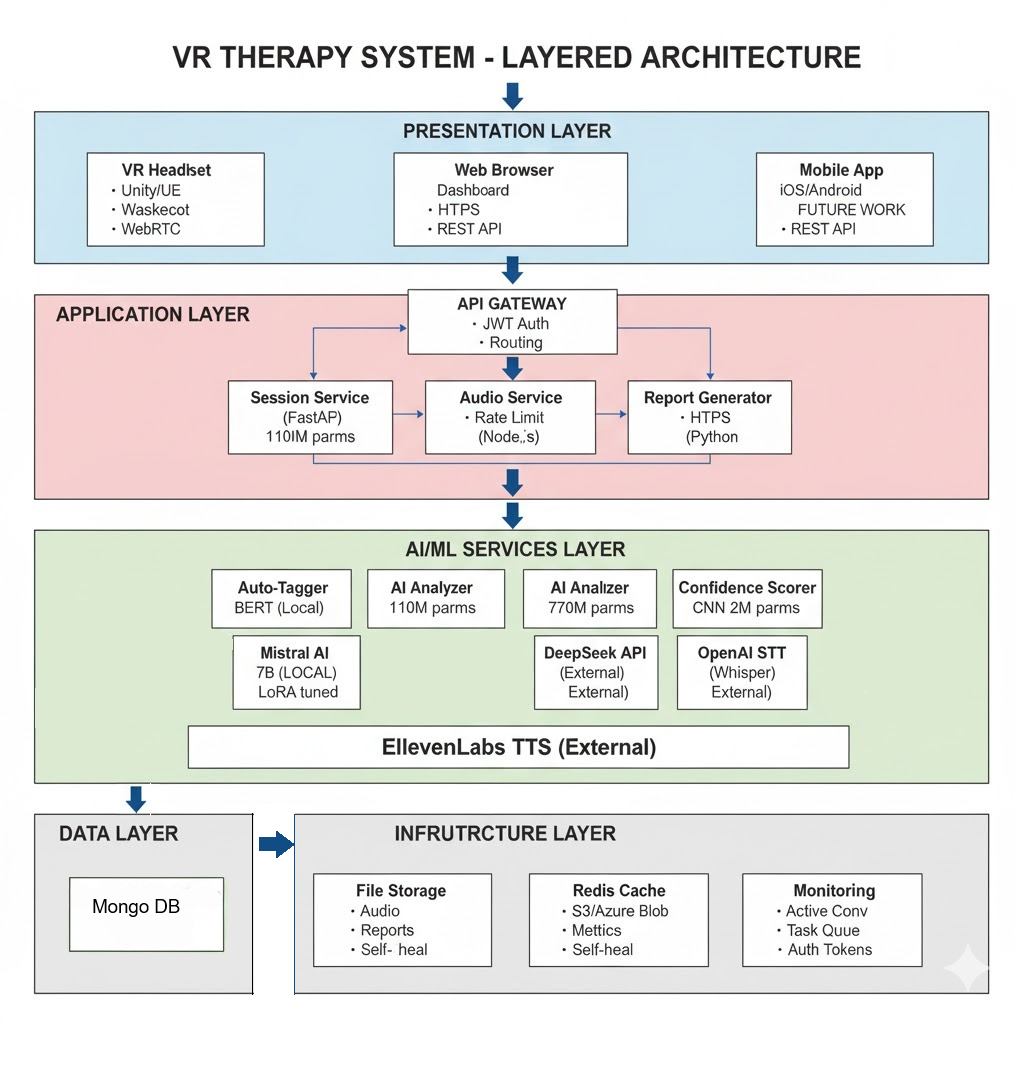
\includegraphics[width=0.9\textwidth]{figures/Layered artitecture.png}
\caption{Layered architecture of VR Therapy System.}
\label{fig:system_architecture}
\end{figure}

\section{Activity Diagram}
The below given activity diagram (Figure \ref{fig:activity_diagram}) is representing the sequential workflow of a complete session. The process begins when a user starts a new session. He's providing the information on issue, intensity, and voice input. The system then enters the AI conversation loop which performs auto-tagging and condition analysis. It selects an appropriate VR simulation and delivers the simulation. It captures post session feedback and scores of the session and then saves the report in the database.

\begin{figure}[H]
    \centering
    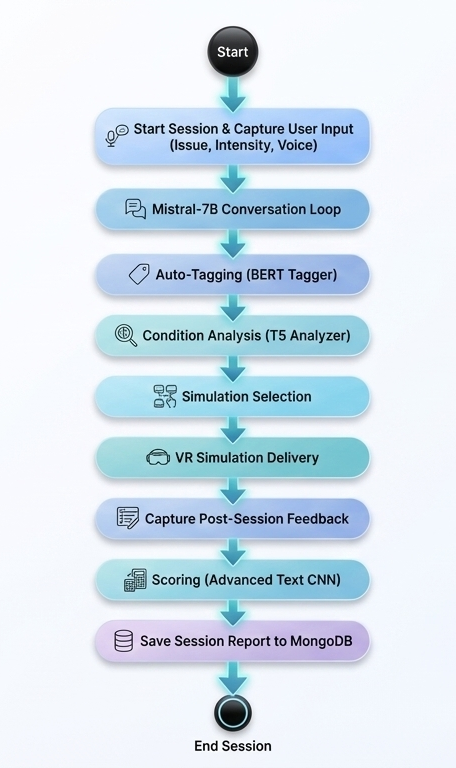
\includegraphics[width=0.75\textwidth]{figures/Activity Diagram.png}
    \caption{Activity diagram of the therapy session workflow.}
    \label{fig:activity_diagram}
\end{figure}

\section{ER Diagram}
The Entity Relationship (ER) diagram (Figure \ref{fig:er_diagram}) is representing the db schema.The User entity is serving as the central point for all of the data relations. The User entity includes attributes such as Name, Email, Age, and Department/Role and represents the individual seeking mental health support. Each and every User can generate multiple chat logs stored in the Chat\_Log entity, which is recording the timestamp, message content and the senders info. The AI\_Model entity is representing the AI engines processing the chat logs with the attributes including the Model Type, Version, and Accuracy Score. Analytical outputs such as Risk Level, Summary Content and the generation dates are stored in the Report entity. Users can schedule the appointments via the Counselling\_Session entity which is conducted by a Counsellor with the Name, Specialization, and Contact Info. Users provide feedback which is recorded in the Feedback entity. It includes Rating, Comments, and Submission Date. 

\begin{figure}[H]
\centering
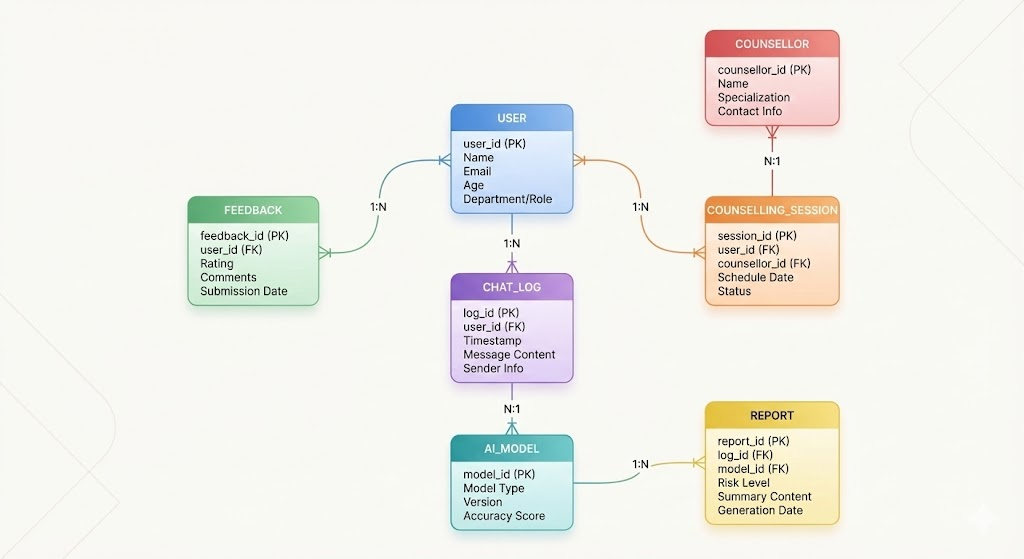
\includegraphics[width=0.99\textwidth]{figures/ER DIAGRAM.png}
\caption{ (ER)Entity Relationship Diagram of VR therapy system.}
\label{fig:er_diagram}
\end{figure}

\section{Class Diagram}

The Class Diagram given below (Figure~\ref{fig:class_diagram}) is providing a representation of the software objects used within our project. It is following the Object-Oriented Programming (OOP) principles and shows the major classes, their attributes, methods, and the relationships that defines the systems behavioral and structural architecture. The given diagram is divided into user-level classes, system logic and analysis classes, therapy and VR simulation classes, and utility or backend management classes.

\paragraph{User-Level Actor Classes}
At the core of the actor hierarchy is the \textbf{User} class which is defining the fundamental properties and functionalities shared by all individuals interacting with our system. This includes general attributes including \textit{UserID}, \textit{Name}, \textit{Email}, and \textit{Password}, as well as methods including \textit{Login()}, \textit{Logout()}, and \textit{UpdateProfile()}. Two special classes extending the base class. The \textbf{Student} (or Client) class represents individuals who are seeking counseling services through our platform. It introduces attributes \textit{StudentID}, \textit{Department}, and \textit{Age} also the methods such as \textit{StartChat()}, \textit{BookSession()}, and \textit{ViewReport()}. The \textbf{Counsellor} class models professional practitioners responsible for guiding therapy sessions. It adds attributes \textit{CounsellorID}, \textit{Specialization}, and \textit{AvailableSlots}, and provides methods including \textit{ViewStudentData()}, \textit{ApproveSession()}, and \textit{WriteSessionNotes()}.

\paragraph{Communication and Interaction Classes}
Central to system interaction is the \textbf{ChatSystem}. It handles the realtime text communication. This class is storing chat data through attributes  \textit{ChatID}, \textit{Timestamp}, and \textit{MessageLog}, and facilitates user engagement through methods that process messages, display system responses, and archive conversation history. For VR-based communication, the system is using a \textbf{VRInteractionManager}. It handles in-environment interactions and user navigation within VR therapy spaces. Audio-based interaction is managed by the \textbf{VoiceProcessor}. It orchestrates voice-related tasks and delegates specific responsibilities to two subordinate components: \textbf{SpeechToText}, which converts audio input into textual data, and \textbf{TextPreprocessor}, which cleans, structures, and prepares text for subsequent ML analysis.

\paragraph{AI and Analysis Layer}
The AI processing layer is encapsulating the several classes that implement machine-learning models and inference procedures. The \textbf{AI\_Analyzer} class is acting as the central intelligence module responsible for interpreting user messages. It maintains the attributes such as \textit{ModelVersion} and \textit{ConfidenceThreshold}. It offers methods to preprocess text, analyze sentiment, detect risk factors, and generate AI responses. Complementing this functionality is the \textbf{AutoTagger}, which is automatically assigning the semantic, emotional, or psychological tags to messages. The tagging is supported by an underlying \textbf{TagModel} which stores the trained model weights and configuration data. For deeper interpretation, the \textbf{ConditionAnalyzer} is evaluating conversation context, infers underlying emotional states, and aids in generating thematic summaries.

\paragraph{Therapy Selection and VR Simulation Classes}
Based on the output of the analytical modules our system determines appropriate actions through the \textbf{TherapySelector} which is maping emotional and behavioral assessments to suitable VR-based interventions. Each VR treatment option is encapsulated in a \textbf{TherapyModule}. It defines environment types, therapeutic goals, and the configurable parameters. Execution of selected therapy modules is managed by the \textbf{SimulationManager}. It controls session timing and in-VR stimuli presentation.

\paragraph{Evaluation and Reporting}
Post-session evaluation is handled by the \textbf{EvaluationManager}. It assesses user feedback, emotional responses, and behavioral changes after a VR therapy experience. Insights from this evaluation process contributing to the generation of comprehensive session reports produced by the \textbf{ReportGenerator}. These reports compile conversation history, analytical results, therapy decisions, and evaluation outcomes into structured formats (such as PDF or JSON). This is enabling both students and counsellors to review progress and outcomes.

\paragraph{Utility, Data Management, and System Support}
Backend operations are supported by several utility classes. The \textbf{SessionManager} oversees the scheduling and administration of both VR and text-based therapy sessions, coordinating interactions between students and counsellors. The \textbf{DatabaseManager} is handling the data persistence and storage operations, including creating, retrieving, updating, and deleting system entities. To ensure the monitoring and debugging, the \textbf{Logger} captures all system events, errors, and activity logs, contributing to the reliability and maintainability of the platform.

\paragraph{Relationships and Multiplicities}
The relationships among these classes reflect the functional workflow of our system. A single User may initiate multiple chat sessions through the ChatSystem, and each chat session is processed by an instance of the AI\_Analyzer. The outputs of the AI\_Analyzer, AutoTagger, and ConditionAnalyzer are used collectively by the TherapySelector and ReportGenerator. Students and Counsellors interact with the SessionManager for booking and approving sessions.VR simulation components engage with both analysis outputs and user interactions. All components depend on the DatabaseManager for persistent storage, and the Logger continuously records system activity across all modules.



\begin{figure}[H]
\centering
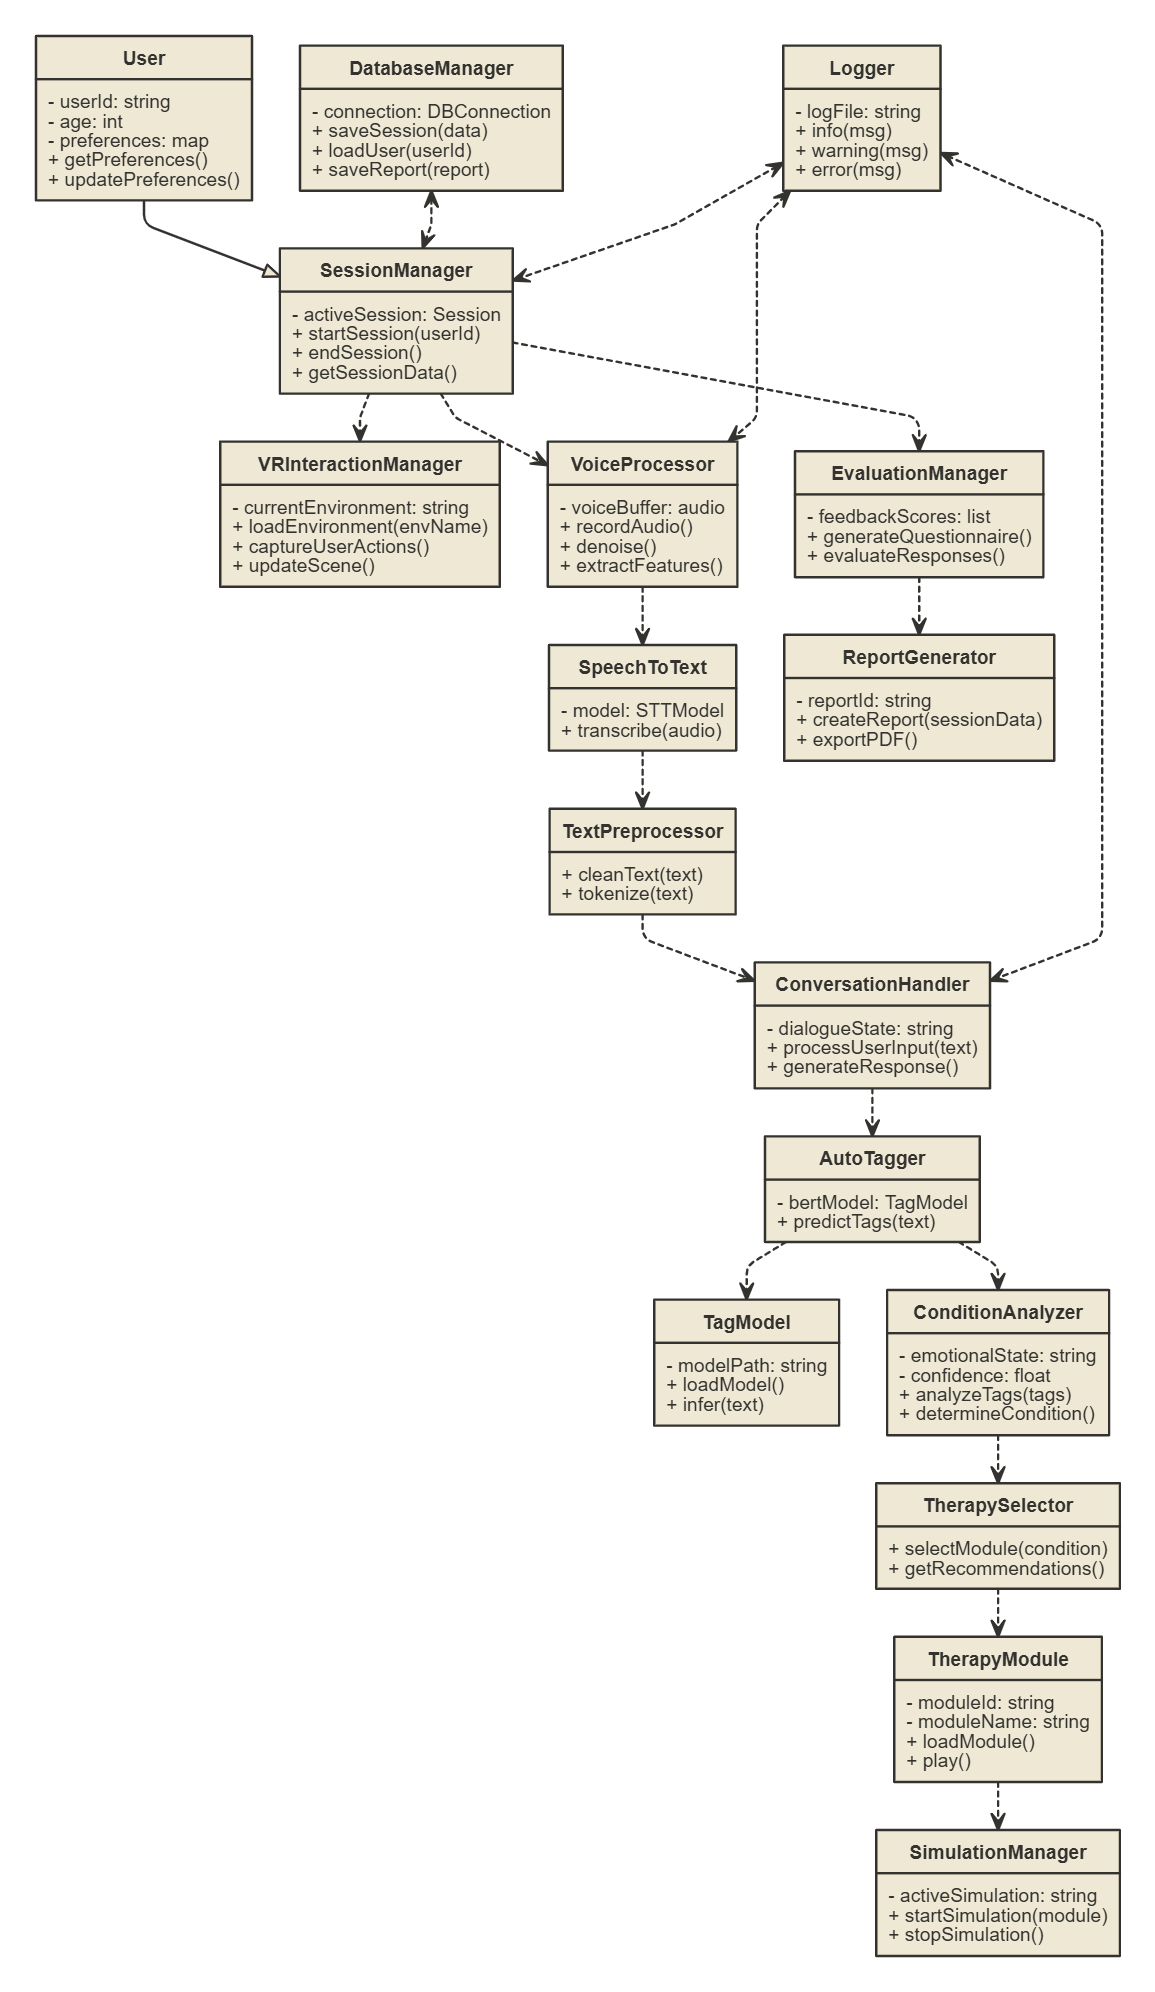
\includegraphics[width=0.85\textwidth]{figures/Class Diagram.png}
\caption{Class Diagram of the VR therapy system.}
\label{fig:class_diagram}
\end{figure}

\section{GUI Design}
The VR frontend is designed for professional and user-friendly interactions. Users provide input on issue type and intensity, and the system recommends simulations such as Relaxation, Exposure Therapy, Cognitive Behavioral Therapy, Mindfulness, and Social Interaction Simulation. Intensity is classified as mild, moderate, hard, or extreme. Post-session feedback is captured for evaluation. The interface provides a simple panel with options to speak, receive AI responses, view recommended simulations, and end the session.

% ---------------------------------------------
% Admin & Dashboard Figures
% ---------------------------------------------
\begin{figure}[H]
    \centering
    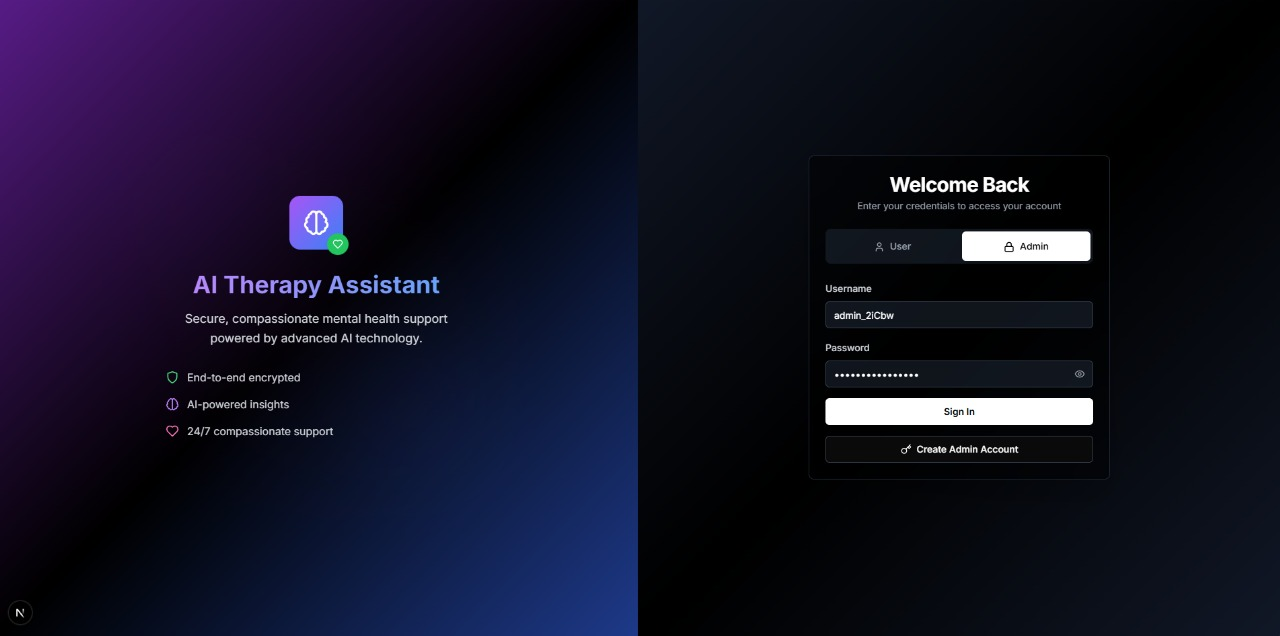
\includegraphics[width=0.85\textwidth]{figures/dashboard.jpg}
    \caption{System Login and Landing Page}
    \label{fig:dashboard}
\end{figure}

\begin{figure}[H]
    \centering
    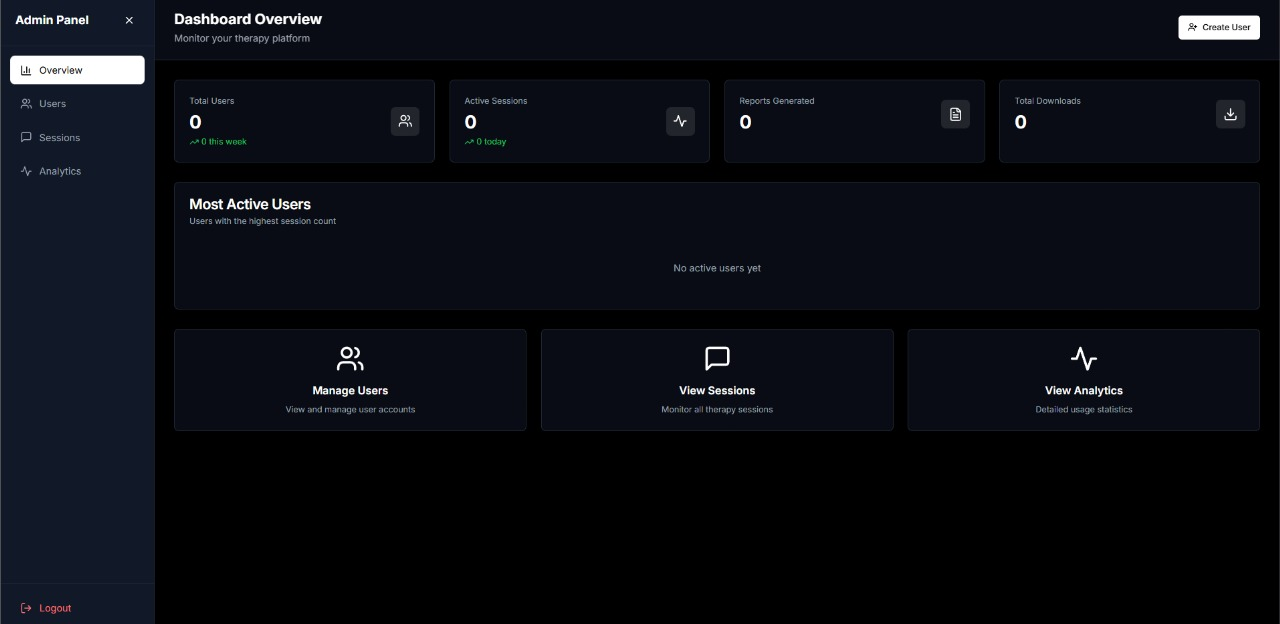
\includegraphics[width=0.85\textwidth]{figures/Admin.jpg}
    \caption{Admin Dashboard Overview and Analytics}
    \label{fig:admin_panel}
\end{figure}

\begin{figure}[H]
    \centering
    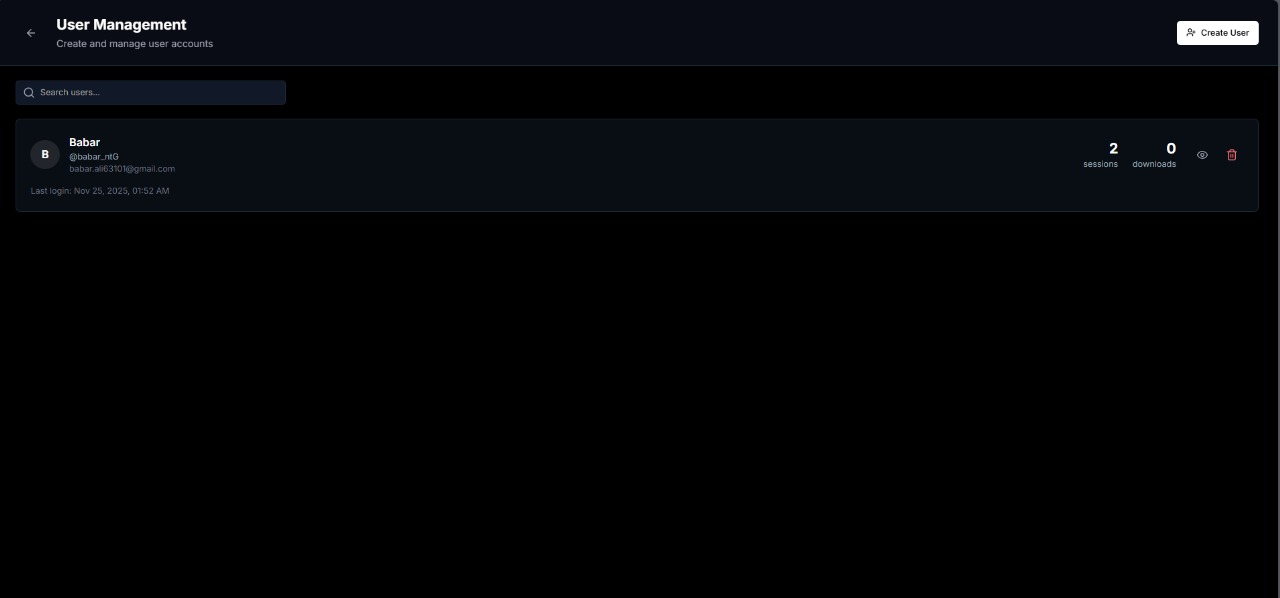
\includegraphics[width=0.85\textwidth]{figures/User Managment.jpg}
    \caption{User Management Interface for Administrators}
    \label{fig:user_mgmt}
\end{figure}

% ---------------------------------------------
% User Interaction Figures
% ---------------------------------------------
\begin{figure}[H]
    \centering
    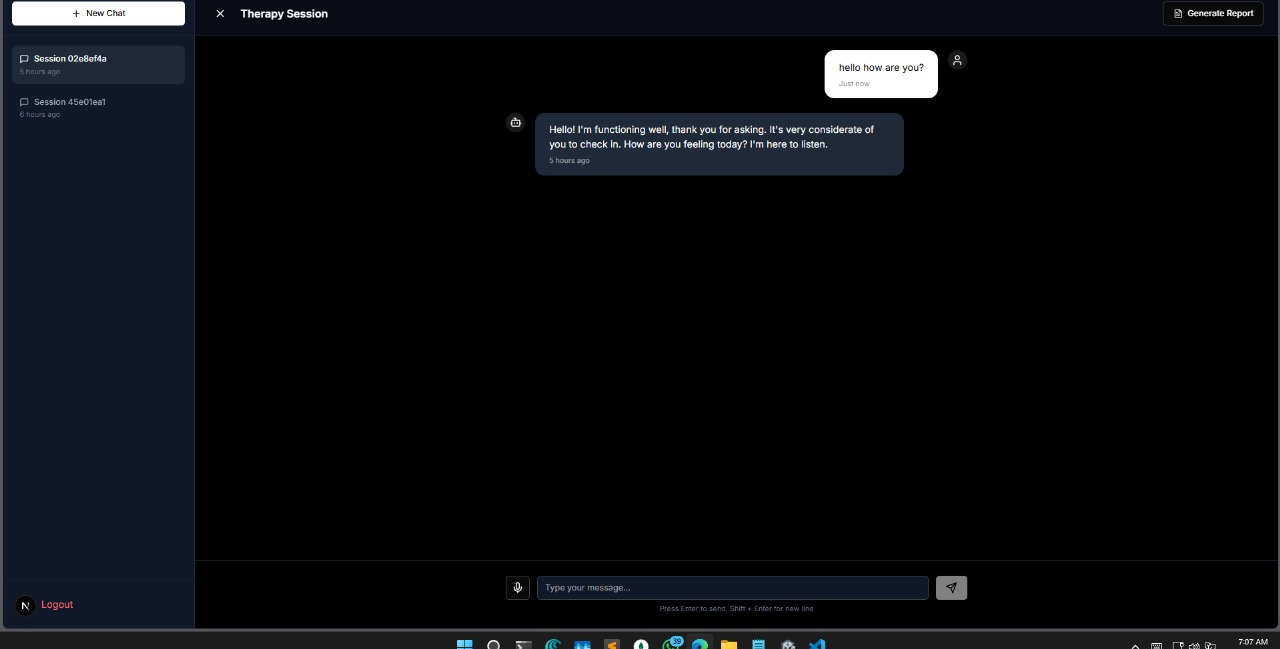
\includegraphics[width=0.85\textwidth]{figures/User Side.jpg}
    \caption{User Chat Interface for Therapy Sessions}
    \label{fig:user_side}
\end{figure}

% ---------------------------------------------
% VR Environment Figures
% ---------------------------------------------
\begin{figure}[H]
    \centering
    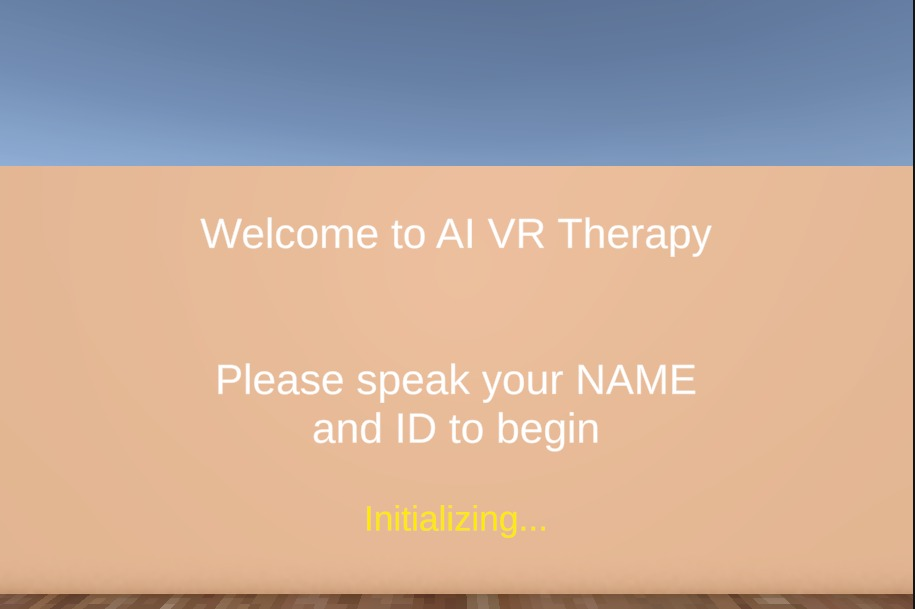
\includegraphics[width=0.85\textwidth]{figures/VR 1ST Scene.jpg}
    \caption{VR Application Initialization and Welcome Screen}
    \label{fig:vr_scene_1}
\end{figure}

\begin{figure}[H]
    \centering
    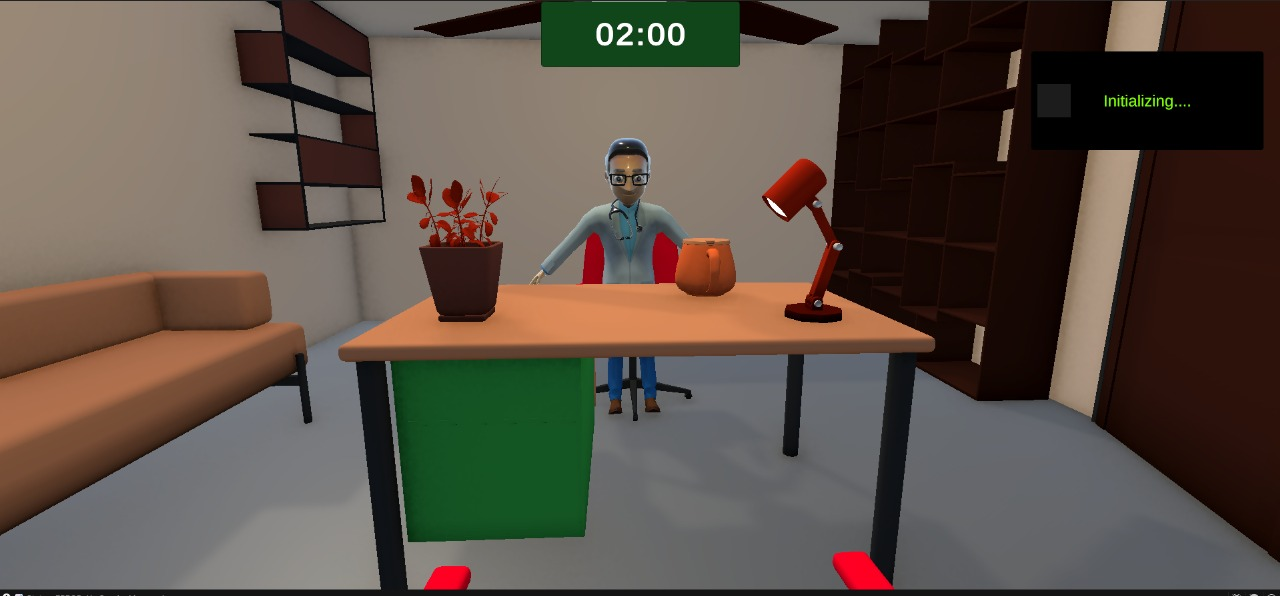
\includegraphics[width=0.85\textwidth]{figures/VR 2ND AND 4TH SCENE.jpg}
    \caption{VR Therapy Room Environment and Simulation}
    \label{fig:vr_scene_2_4}
\end{figure}

\section{Summary}
This chapter presented the system analysis and design of the VR-based mental health therapy platform. It described the architecture, workflow, ERD, class diagram, and GUI design. The activity diagram illustrates the therapy session flow, the ERD details all entities and their relationships with the User as the central point, and the class diagram shows core actor classes, system logic classes, and their interactions. Together, these models provide a detailed blueprint for implementing the system in the next chapter.
